Since the armpit microbiome only contains two genera of bacteria, the relative abundance of one defines the other.
Malodor is caused mainly by Corynebacteria. 
The analysis focuses on the relative abundance of this genus.
The abundance of the Staphylococcus genus is simply $100\% - RGA$ of Corynebacteria.

\subsubsection{Basic statistics}
Table \ref{tab:BacteriaStatistics} contains the basic statistics of the relative distributions of the different bacteria species.
The RGA shows a strongly skewed distribution. 
The relative Corynebacteria abundance is very low (only 3.2\%) for at least half of the patients.
Nevertheless, the armpit microbiome relative concentration of Corynebacteria can be as high as 97\%. This is visualized in figure \ref{fig:boxplot_cory}.
\begin{figure}
    \centering
     \resizebox{\hsize}{!}{%
       % Created by tikzDevice version 0.12.3 on 2019-12-11 20:53:26
% !TEX encoding = UTF-8 Unicode
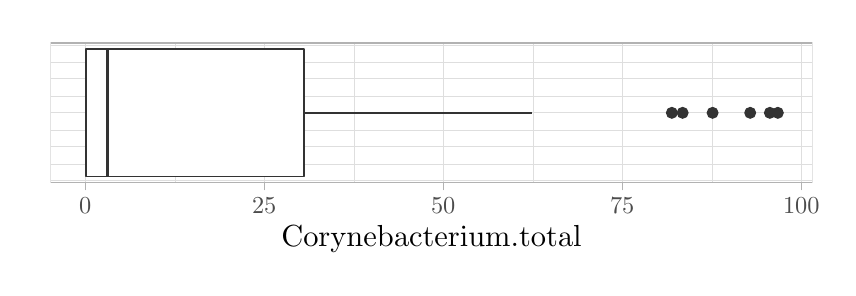
\begin{tikzpicture}[x=1pt,y=1pt]
\definecolor{fillColor}{RGB}{255,255,255}
\path[use as bounding box,fill=fillColor,fill opacity=0.00] (0,0) rectangle (289.08, 86.72);
\begin{scope}
\path[clip] (  0.00,  0.00) rectangle (289.08, 86.72);
\definecolor{drawColor}{RGB}{255,255,255}
\definecolor{fillColor}{RGB}{255,255,255}

\path[draw=drawColor,line width= 0.6pt,line join=round,line cap=round,fill=fillColor] (  0.00,  0.00) rectangle (289.08, 86.72);
\end{scope}
\begin{scope}
\path[clip] (  8.25, 30.69) rectangle (283.58, 81.22);
\definecolor{fillColor}{RGB}{255,255,255}

\path[fill=fillColor] (  8.25, 30.69) rectangle (283.58, 81.22);
\definecolor{drawColor}{gray}{0.87}

\path[draw=drawColor,line width= 0.1pt,line join=round] (  8.25, 37.58) --
	(283.58, 37.58);

\path[draw=drawColor,line width= 0.1pt,line join=round] (  8.25, 49.83) --
	(283.58, 49.83);

\path[draw=drawColor,line width= 0.1pt,line join=round] (  8.25, 62.08) --
	(283.58, 62.08);

\path[draw=drawColor,line width= 0.1pt,line join=round] (  8.25, 74.33) --
	(283.58, 74.33);

\path[draw=drawColor,line width= 0.1pt,line join=round] ( 53.11, 30.69) --
	( 53.11, 81.22);

\path[draw=drawColor,line width= 0.1pt,line join=round] (117.81, 30.69) --
	(117.81, 81.22);

\path[draw=drawColor,line width= 0.1pt,line join=round] (182.50, 30.69) --
	(182.50, 81.22);

\path[draw=drawColor,line width= 0.1pt,line join=round] (247.19, 30.69) --
	(247.19, 81.22);

\path[draw=drawColor,line width= 0.3pt,line join=round] (  8.25, 31.45) --
	(283.58, 31.45);

\path[draw=drawColor,line width= 0.3pt,line join=round] (  8.25, 43.70) --
	(283.58, 43.70);

\path[draw=drawColor,line width= 0.3pt,line join=round] (  8.25, 55.95) --
	(283.58, 55.95);

\path[draw=drawColor,line width= 0.3pt,line join=round] (  8.25, 68.21) --
	(283.58, 68.21);

\path[draw=drawColor,line width= 0.3pt,line join=round] (  8.25, 80.46) --
	(283.58, 80.46);

\path[draw=drawColor,line width= 0.3pt,line join=round] ( 20.77, 30.69) --
	( 20.77, 81.22);

\path[draw=drawColor,line width= 0.3pt,line join=round] ( 85.46, 30.69) --
	( 85.46, 81.22);

\path[draw=drawColor,line width= 0.3pt,line join=round] (150.15, 30.69) --
	(150.15, 81.22);

\path[draw=drawColor,line width= 0.3pt,line join=round] (214.85, 30.69) --
	(214.85, 81.22);

\path[draw=drawColor,line width= 0.3pt,line join=round] (279.54, 30.69) --
	(279.54, 81.22);
\definecolor{drawColor}{gray}{0.20}
\definecolor{fillColor}{gray}{0.20}

\path[draw=drawColor,line width= 0.4pt,line join=round,line cap=round,fill=fillColor] (268.19, 55.95) circle (  1.96);

\path[draw=drawColor,line width= 0.4pt,line join=round,line cap=round,fill=fillColor] (232.77, 55.95) circle (  1.96);

\path[draw=drawColor,line width= 0.4pt,line join=round,line cap=round,fill=fillColor] (261.08, 55.95) circle (  1.96);

\path[draw=drawColor,line width= 0.4pt,line join=round,line cap=round,fill=fillColor] (247.49, 55.95) circle (  1.96);

\path[draw=drawColor,line width= 0.4pt,line join=round,line cap=round,fill=fillColor] (271.06, 55.95) circle (  1.96);

\path[draw=drawColor,line width= 0.4pt,line join=round,line cap=round,fill=fillColor] (236.67, 55.95) circle (  1.96);

\path[draw=drawColor,line width= 0.6pt,line join=round] ( 99.89, 55.95) -- (182.12, 55.95);

\path[draw=drawColor,line width= 0.6pt,line join=round] ( 21.13, 55.95) -- ( 20.77, 55.95);
\definecolor{fillColor}{RGB}{255,255,255}

\path[draw=drawColor,line width= 0.6pt,line join=round,line cap=round,fill=fillColor] ( 99.89, 32.98) --
	( 21.13, 32.98) --
	( 21.13, 78.93) --
	( 99.89, 78.93) --
	( 99.89, 32.98) --
	cycle;

\path[draw=drawColor,line width= 1.1pt,line join=round] ( 29.00, 32.98) -- ( 29.00, 78.93);
\definecolor{drawColor}{gray}{0.70}

\path[draw=drawColor,line width= 0.6pt,line join=round,line cap=round] (  8.25, 30.69) rectangle (283.58, 81.22);
\end{scope}
\begin{scope}
\path[clip] (  0.00,  0.00) rectangle (289.08, 86.72);
\definecolor{drawColor}{gray}{0.70}

\path[draw=drawColor,line width= 0.3pt,line join=round] ( 20.77, 27.94) --
	( 20.77, 30.69);

\path[draw=drawColor,line width= 0.3pt,line join=round] ( 85.46, 27.94) --
	( 85.46, 30.69);

\path[draw=drawColor,line width= 0.3pt,line join=round] (150.15, 27.94) --
	(150.15, 30.69);

\path[draw=drawColor,line width= 0.3pt,line join=round] (214.85, 27.94) --
	(214.85, 30.69);

\path[draw=drawColor,line width= 0.3pt,line join=round] (279.54, 27.94) --
	(279.54, 30.69);
\end{scope}
\begin{scope}
\path[clip] (  0.00,  0.00) rectangle (289.08, 86.72);
\definecolor{drawColor}{gray}{0.30}

\node[text=drawColor,anchor=base,inner sep=0pt, outer sep=0pt, scale=  0.88] at ( 20.77, 19.68) {0};

\node[text=drawColor,anchor=base,inner sep=0pt, outer sep=0pt, scale=  0.88] at ( 85.46, 19.68) {25};

\node[text=drawColor,anchor=base,inner sep=0pt, outer sep=0pt, scale=  0.88] at (150.15, 19.68) {50};

\node[text=drawColor,anchor=base,inner sep=0pt, outer sep=0pt, scale=  0.88] at (214.85, 19.68) {75};

\node[text=drawColor,anchor=base,inner sep=0pt, outer sep=0pt, scale=  0.88] at (279.54, 19.68) {100};
\end{scope}
\begin{scope}
\path[clip] (  0.00,  0.00) rectangle (289.08, 86.72);
\definecolor{drawColor}{RGB}{0,0,0}

\node[text=drawColor,anchor=base,inner sep=0pt, outer sep=0pt, scale=  1.10] at (145.91,  7.64) {Corynebacterium.total};
\end{scope}
\end{tikzpicture}

    }
    \caption{Boxplot of the relative abundances of the Corynebacteria genus in all 39 observations}
    \label{fig:boxplot_cory}
\end{figure}

Within the same genus, the skewness of the data is clear from the second part of the table.
The \textit{Staphylococcus} species 2, 3 and 4 are completely absent in at least half the samples. Nevertheless, the RSA of \textit{Staphylococcus.2} can reach up to 89.7\%.

% Table created by stargazer v.5.2.2 by Marek Hlavac, Harvard University. E-mail: hlavac at fas.harvard.edu
% Date and time: za, dec 07, 2019 - 17:08:05
\begin{table*}[t] \centering 

\begin{tabular}{@{\extracolsep{5pt}} lccccc} 
\\[-1.8ex]\hline 
\hline \\[-1.8ex] 
Genus & mean [\%] & median [\%] & sd [\%] & min [\%] & max [\%]\\ 
\hline \\[-1.8ex] 
Corynebacterium.total & 21 & 3.2 & 33 & 0 & 96.7 \\ 
Staphylococcus.total & 79 & 96.8 & 33 & 3.3 & 100 \\ 
\hline\\
Species  & mean [\%] & median [\%] & sd [\%] & min [\%] & max [\%]\\ 
\hline \\
Corynebacterium.1 & 6.6 & 0.2 & 20.1 & 0 & 96.2 \\ 
Corynebacterium.2 & 11.7 & 0.2 & 25.4 & 0 & 87.2 \\ 
Corynebacterium.3 & 1.4 & 0 & 5 & 0 & 30.2 \\ 
Corynebacterium.4 & 1.2 & 0 & 3.9 & 0 & 18.4 \\ 
Staphylococcus.1 & 71.2 & 93.7 & 36.2 & 1.2 & 100 \\ 
Staphylococcus.2 & 6.3 & 0 & 20.1 & 0 & 89.7 \\ 
Staphylococcus.3 & 0.5 & 0 & 1.4 & 0 & 6.7 \\ 
Staphylococcus.4 & 1 & 0 & 3.6 & 0 & 21.6 \\ 
\hline \\[-1.8ex] 
\end{tabular} 
  \caption{Relative abundance statistics for both genera and all species\label{tab:BacteriaStatistics} \todo{JAL}{Uniform formatting numbers}} 
\end{table*} 


\subsubsection{Age as a categorical variable \label{sec:AgeCategorical}}
Due to the relatively low number of observations, it was chosen to deviate from the original plan to divide the patients in 4 categories divided at 30, 40 en 50 years old.
This resulted in categories containing a very low number of observations. 
This would have yielded the power of the statistical tests undesirably low. \todo{All}{Is this correct? Is this the best way to put it? }
Instead, the patients were split in 2 age categories: \textit{40 and younger} and \textit{over 40}.
The age of 40 years is chosen because:
\begin{itemize}
    \item The mean age of a Belgian is 40.8 years \footnote{Census Belgi\"e, 2011 -  \texttt{https://www.census2011.be/
    data/fresult/age-avg\_nl.html}}.
    \item 40 is close to half of the oldest patient age and the mean participant age.
\end{itemize}

The difference in RGA of Corynebacteria can be observed in figure \ref{fig:BoxplotAge} and from table \ref{tab:CoryStats_AgeCat}.
For most people of maximum 40 years old in this data set, a lower RGA (<10\%) of Corynebacteria is observed (with 4 exceptions). 
The distribution of RGA of Corynebacteria for people over 40 years old shows more variability, the IQR is higher.
The center of this distribution (both the median and the mean) is higher.
The (two-sided) WMW-test indicates a p-value < 0.01, indicating that $H_0$ (no location shift between category \textit{'40 or younger'} and category \textit{'over 40'}) should be rejected.

\begin{figure}
    \centering
     \resizebox{\hsize}{!}{%
       \input{images/plot_age.tex}
    }
    \caption{Boxplot of Corybacteria RGA per age category. The points indicate the individual observations. Grey markers indicate the mean for both groups.}
    \label{fig:BoxplotAge}
\end{figure}


Apart from the patient's age, two other patient characteristics are known:
\begin{enumerate}
    \item Whether the patient's BMI is over 25.
    \item The patient's gender.
\end{enumerate}


% Table created by stargazer v.5.2.2 by Marek Hlavac, Harvard University. E-mail: hlavac at fas.harvard.edu
% Date and time: Wed, Dec 11, 2019 - 20:53:29
\begin{table}[!htbp] \centering 
  \caption{} 
  \label{} 
\begin{tabular}{@{\extracolsep{5pt}} cccccccc} 
\\[-1.8ex]\hline 
\hline \\[-1.8ex] 
Agecat & n & mean & min & median & max & n\_present & percentage\_present \\ 
\hline \\[-1.8ex] 
1 & 27 & 9 & 0 & 1.6 & 83.4 & 21 & 77.8 \\ 
2 & 12 & 47.9 & 0 & 41.7 & 96.7 & 11 & 91.7 \\ 
\hline \\[-1.8ex] 
\end{tabular} 
\end{table} 


Before concluding we observed a location shift between the relative bacteria genus abundances in the armpit microbiome in different age categories, 
we wish to investigate the possible influence the two other mentioned parameters may have.
Secondly, we want to investigate if there is a significant difference between both age categories in BMI or gender composition.

In table \ref{tab:ageDistrAfterDiscr}, the distribution of the patients in the categories is shown.

% Table created by stargazer v.5.2.2 by Marek Hlavac, Harvard University. E-mail: hlavac at fas.harvard.edu
% Date and time: Wed, Dec 11, 2019 - 20:53:29
\begin{table}[!htbp] \centering 
  \caption{} 
  \label{} 
\begin{tabular}{@{\extracolsep{5pt}} cccc} 
\\[-1.8ex]\hline 
\hline \\[-1.8ex] 
BMI & Gender & 40 or younger & over 40 \\ 
\hline \\[-1.8ex] 
1 & 1 & 14 & 4 \\ 
1 & 2 & 6 & 2 \\ 
2 & 1 & 5 & 1 \\ 
2 & 2 & 2 & 5 \\ 
\hline \\[-1.8ex] 
\end{tabular} 
\end{table} 



\begin{figure}
    \centering
     \resizebox{\hsize}{!}{%
       % Created by tikzDevice version 0.12.3 on 2019-12-11 20:53:31
% !TEX encoding = UTF-8 Unicode
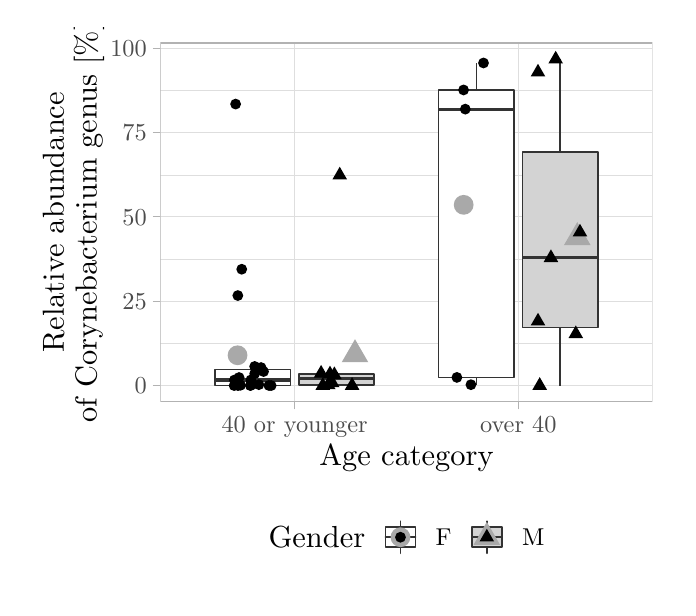
\begin{tikzpicture}[x=1pt,y=1pt]
\definecolor{fillColor}{RGB}{255,255,255}
\path[use as bounding box,fill=fillColor,fill opacity=0.00] (0,0) rectangle (231.26,202.36);
\begin{scope}
\path[clip] (  0.00,  0.00) rectangle (231.26,202.36);
\definecolor{drawColor}{RGB}{255,255,255}
\definecolor{fillColor}{RGB}{255,255,255}

\path[draw=drawColor,line width= 0.6pt,line join=round,line cap=round,fill=fillColor] (  0.00,  0.00) rectangle (231.26,202.36);
\end{scope}
\begin{scope}
\path[clip] ( 47.99, 67.14) rectangle (225.76,196.86);
\definecolor{fillColor}{RGB}{255,255,255}

\path[fill=fillColor] ( 47.99, 67.14) rectangle (225.76,196.86);
\definecolor{drawColor}{gray}{0.87}

\path[draw=drawColor,line width= 0.1pt,line join=round] ( 47.99, 88.28) --
	(225.76, 88.28);

\path[draw=drawColor,line width= 0.1pt,line join=round] ( 47.99,118.75) --
	(225.76,118.75);

\path[draw=drawColor,line width= 0.1pt,line join=round] ( 47.99,149.23) --
	(225.76,149.23);

\path[draw=drawColor,line width= 0.1pt,line join=round] ( 47.99,179.71) --
	(225.76,179.71);

\path[draw=drawColor,line width= 0.3pt,line join=round] ( 47.99, 73.04) --
	(225.76, 73.04);

\path[draw=drawColor,line width= 0.3pt,line join=round] ( 47.99,103.52) --
	(225.76,103.52);

\path[draw=drawColor,line width= 0.3pt,line join=round] ( 47.99,133.99) --
	(225.76,133.99);

\path[draw=drawColor,line width= 0.3pt,line join=round] ( 47.99,164.47) --
	(225.76,164.47);

\path[draw=drawColor,line width= 0.3pt,line join=round] ( 47.99,194.95) --
	(225.76,194.95);

\path[draw=drawColor,line width= 0.3pt,line join=round] ( 96.47, 67.14) --
	( 96.47,196.86);

\path[draw=drawColor,line width= 0.3pt,line join=round] (177.28, 67.14) --
	(177.28,196.86);

\path[] ( 81.32,115.07) circle (  1.96);

\path[] ( 81.32,105.56) circle (  1.96);

\path[] ( 81.32,174.75) circle (  1.96);
\definecolor{drawColor}{gray}{0.20}

\path[draw=drawColor,line width= 0.6pt,line join=round] ( 81.32, 78.82) -- ( 81.32, 79.94);

\path[draw=drawColor,line width= 0.6pt,line join=round] ( 81.32, 73.11) -- ( 81.32, 73.04);

\path[draw=drawColor,line width= 0.6pt,line join=round,line cap=round,fill=fillColor] ( 67.69, 78.82) --
	( 67.69, 73.11) --
	( 94.96, 73.11) --
	( 94.96, 78.82) --
	( 67.69, 78.82) --
	cycle;

\path[draw=drawColor,line width= 1.1pt,line join=round] ( 67.69, 75.04) -- ( 94.96, 75.04);

\path[] (111.63,149.06) circle (  1.96);

\path[draw=drawColor,line width= 0.6pt,line join=round] (111.63, 77.24) -- (111.63, 77.44);

\path[draw=drawColor,line width= 0.6pt,line join=round] (111.63, 73.21) -- (111.63, 73.04);
\definecolor{fillColor}{RGB}{211,211,211}

\path[draw=drawColor,line width= 0.6pt,line join=round,line cap=round,fill=fillColor] ( 97.99, 77.24) --
	( 97.99, 73.21) --
	(125.26, 73.21) --
	(125.26, 77.24) --
	( 97.99, 77.24) --
	cycle;

\path[draw=drawColor,line width= 1.1pt,line join=round] ( 97.99, 75.44) -- (125.26, 75.44);

\path[draw=drawColor,line width= 0.6pt,line join=round] (162.13,179.85) -- (162.13,189.60);

\path[draw=drawColor,line width= 0.6pt,line join=round] (162.13, 75.98) -- (162.13, 73.35);
\definecolor{fillColor}{RGB}{255,255,255}

\path[draw=drawColor,line width= 0.6pt,line join=round,line cap=round,fill=fillColor] (148.49,179.85) --
	(148.49, 75.98) --
	(175.77, 75.98) --
	(175.77,179.85) --
	(148.49,179.85) --
	cycle;

\path[draw=drawColor,line width= 1.1pt,line join=round] (148.49,172.92) -- (175.77,172.92);

\path[draw=drawColor,line width= 0.6pt,line join=round] (192.43,157.34) -- (192.43,190.96);

\path[draw=drawColor,line width= 0.6pt,line join=round] (192.43, 93.99) -- (192.43, 73.04);
\definecolor{fillColor}{RGB}{211,211,211}

\path[draw=drawColor,line width= 0.6pt,line join=round,line cap=round,fill=fillColor] (178.80,157.34) --
	(178.80, 93.99) --
	(206.07, 93.99) --
	(206.07,157.34) --
	(178.80,157.34) --
	cycle;

\path[draw=drawColor,line width= 1.1pt,line join=round] (178.80,119.20) -- (206.07,119.20);
\definecolor{fillColor}{RGB}{169,169,169}

\path[fill=fillColor] (118.28, 89.78) --
	(123.08, 81.46) --
	(113.47, 81.46) --
	cycle;

\path[fill=fillColor] ( 75.84, 83.98) circle (  3.57);

\path[fill=fillColor] (198.60,132.10) --
	(203.41,123.78) --
	(193.79,123.78) --
	cycle;

\path[fill=fillColor] (157.55,138.34) circle (  3.57);
\definecolor{fillColor}{RGB}{0,0,0}

\path[fill=fillColor] (106.64, 76.09) --
	(109.28, 71.51) --
	(104.00, 71.51) --
	cycle;

\path[fill=fillColor] (110.06, 77.01) --
	(112.70, 72.43) --
	(107.42, 72.43) --
	cycle;

\path[fill=fillColor] (106.03, 80.49) --
	(108.68, 75.92) --
	(103.39, 75.92) --
	cycle;

\path[fill=fillColor] (117.22, 76.09) --
	(119.87, 71.51) --
	(114.58, 71.51) --
	cycle;

\path[fill=fillColor] (108.60, 76.31) --
	(111.24, 71.74) --
	(105.95, 71.74) --
	cycle;

\path[fill=fillColor] (112.76,152.11) --
	(115.40,147.53) --
	(110.12,147.53) --
	cycle;

\path[fill=fillColor] (109.24, 80.22) --
	(111.88, 75.64) --
	(106.59, 75.64) --
	cycle;

\path[fill=fillColor] (110.82, 79.97) --
	(113.46, 75.39) --
	(108.17, 75.39) --
	cycle;

\path[fill=fillColor] ( 76.40, 75.94) circle (  1.96);

\path[fill=fillColor] ( 76.01, 73.04) circle (  1.96);

\path[fill=fillColor] ( 84.34, 79.54) circle (  1.96);

\path[fill=fillColor] ( 87.98, 73.04) circle (  1.96);

\path[fill=fillColor] ( 77.35,115.07) circle (  1.96);

\path[fill=fillColor] ( 74.70, 75.04) circle (  1.96);

\path[fill=fillColor] ( 75.94,105.56) circle (  1.96);

\path[fill=fillColor] ( 80.66, 75.07) circle (  1.96);

\path[fill=fillColor] ( 76.92, 73.15) circle (  1.96);

\path[fill=fillColor] ( 85.23, 78.10) circle (  1.96);

\path[fill=fillColor] ( 80.59, 73.15) circle (  1.96);

\path[fill=fillColor] ( 82.02, 79.94) circle (  1.96);

\path[fill=fillColor] ( 87.17, 73.07) circle (  1.96);

\path[fill=fillColor] ( 75.14,174.75) circle (  1.96);

\path[fill=fillColor] ( 80.47, 73.04) circle (  1.96);

\path[fill=fillColor] ( 74.61, 73.04) circle (  1.96);

\path[fill=fillColor] ( 75.44, 74.29) circle (  1.96);

\path[fill=fillColor] ( 82.03, 77.35) circle (  1.96);

\path[fill=fillColor] ( 83.54, 73.37) circle (  1.96);

\path[fill=fillColor] (189.08,122.25) --
	(191.72,117.68) --
	(186.44,117.68) --
	cycle;

\path[fill=fillColor] (185.02, 76.09) --
	(187.66, 71.51) --
	(182.37, 71.51) --
	cycle;

\path[fill=fillColor] (184.40,189.31) --
	(187.04,184.73) --
	(181.76,184.73) --
	cycle;

\path[fill=fillColor] (184.41, 99.33) --
	(187.05, 94.75) --
	(181.76, 94.75) --
	cycle;

\path[fill=fillColor] (198.07, 94.77) --
	(200.71, 90.19) --
	(195.43, 90.19) --
	cycle;

\path[fill=fillColor] (199.57,131.48) --
	(202.22,126.90) --
	(196.93,126.90) --
	cycle;

\path[fill=fillColor] (190.79,194.01) --
	(193.44,189.43) --
	(188.15,189.43) --
	cycle;

\path[fill=fillColor] (164.71,189.60) circle (  1.96);

\path[fill=fillColor] (158.13,172.92) circle (  1.96);

\path[fill=fillColor] (155.10, 75.98) circle (  1.96);

\path[fill=fillColor] (157.51,179.85) circle (  1.96);

\path[fill=fillColor] (160.17, 73.35) circle (  1.96);
\definecolor{drawColor}{gray}{0.70}

\path[draw=drawColor,line width= 0.6pt,line join=round,line cap=round] ( 47.99, 67.14) rectangle (225.76,196.86);
\end{scope}
\begin{scope}
\path[clip] (  0.00,  0.00) rectangle (231.26,202.36);
\definecolor{drawColor}{gray}{0.30}

\node[text=drawColor,anchor=base east,inner sep=0pt, outer sep=0pt, scale=  0.88] at ( 43.04, 70.01) {0};

\node[text=drawColor,anchor=base east,inner sep=0pt, outer sep=0pt, scale=  0.88] at ( 43.04,100.48) {25};

\node[text=drawColor,anchor=base east,inner sep=0pt, outer sep=0pt, scale=  0.88] at ( 43.04,130.96) {50};

\node[text=drawColor,anchor=base east,inner sep=0pt, outer sep=0pt, scale=  0.88] at ( 43.04,161.44) {75};

\node[text=drawColor,anchor=base east,inner sep=0pt, outer sep=0pt, scale=  0.88] at ( 43.04,191.92) {100};
\end{scope}
\begin{scope}
\path[clip] (  0.00,  0.00) rectangle (231.26,202.36);
\definecolor{drawColor}{gray}{0.70}

\path[draw=drawColor,line width= 0.3pt,line join=round] ( 45.24, 73.04) --
	( 47.99, 73.04);

\path[draw=drawColor,line width= 0.3pt,line join=round] ( 45.24,103.52) --
	( 47.99,103.52);

\path[draw=drawColor,line width= 0.3pt,line join=round] ( 45.24,133.99) --
	( 47.99,133.99);

\path[draw=drawColor,line width= 0.3pt,line join=round] ( 45.24,164.47) --
	( 47.99,164.47);

\path[draw=drawColor,line width= 0.3pt,line join=round] ( 45.24,194.95) --
	( 47.99,194.95);
\end{scope}
\begin{scope}
\path[clip] (  0.00,  0.00) rectangle (231.26,202.36);
\definecolor{drawColor}{gray}{0.70}

\path[draw=drawColor,line width= 0.3pt,line join=round] ( 96.47, 64.39) --
	( 96.47, 67.14);

\path[draw=drawColor,line width= 0.3pt,line join=round] (177.28, 64.39) --
	(177.28, 67.14);
\end{scope}
\begin{scope}
\path[clip] (  0.00,  0.00) rectangle (231.26,202.36);
\definecolor{drawColor}{gray}{0.30}

\node[text=drawColor,anchor=base,inner sep=0pt, outer sep=0pt, scale=  0.88] at ( 96.47, 56.13) {40 or younger};

\node[text=drawColor,anchor=base,inner sep=0pt, outer sep=0pt, scale=  0.88] at (177.28, 56.13) {over 40};
\end{scope}
\begin{scope}
\path[clip] (  0.00,  0.00) rectangle (231.26,202.36);
\definecolor{drawColor}{RGB}{0,0,0}

\node[text=drawColor,anchor=base,inner sep=0pt, outer sep=0pt, scale=  1.10] at (136.88, 44.09) {Age category};
\end{scope}
\begin{scope}
\path[clip] (  0.00,  0.00) rectangle (231.26,202.36);
\definecolor{drawColor}{RGB}{0,0,0}

\node[text=drawColor,rotate= 90.00,anchor=base,inner sep=0pt, outer sep=0pt, scale=  1.10] at ( 13.08,132.00) {Relative abundance };

\node[text=drawColor,rotate= 90.00,anchor=base,inner sep=0pt, outer sep=0pt, scale=  1.10] at ( 24.96,132.00) { of Corynebacterium genus [\%]};
\end{scope}
\begin{scope}
\path[clip] (  0.00,  0.00) rectangle (231.26,202.36);
\definecolor{fillColor}{RGB}{255,255,255}

\path[fill=fillColor] ( 81.55,  5.50) rectangle (192.20, 30.95);
\end{scope}
\begin{scope}
\path[clip] (  0.00,  0.00) rectangle (231.26,202.36);
\definecolor{drawColor}{RGB}{0,0,0}

\node[text=drawColor,anchor=base west,inner sep=0pt, outer sep=0pt, scale=  1.10] at ( 87.05, 14.44) {Gender};
\end{scope}
\begin{scope}
\path[clip] (  0.00,  0.00) rectangle (231.26,202.36);
\definecolor{fillColor}{RGB}{255,255,255}

\path[fill=fillColor] (127.49, 11.00) rectangle (141.94, 25.45);
\end{scope}
\begin{scope}
\path[clip] (  0.00,  0.00) rectangle (231.26,202.36);
\definecolor{drawColor}{gray}{0.20}

\path[draw=drawColor,line width= 0.6pt,line join=round,line cap=round] (134.71, 12.45) --
	(134.71, 14.61);

\path[draw=drawColor,line width= 0.6pt,line join=round,line cap=round] (134.71, 21.84) --
	(134.71, 24.01);
\definecolor{fillColor}{RGB}{255,255,255}

\path[draw=drawColor,line width= 0.6pt,line join=round,line cap=round,fill=fillColor] (129.29, 14.61) rectangle (140.13, 21.84);

\path[draw=drawColor,line width= 0.6pt,line join=round,line cap=round] (129.29, 18.23) --
	(140.13, 18.23);
\end{scope}
\begin{scope}
\path[clip] (  0.00,  0.00) rectangle (231.26,202.36);
\definecolor{fillColor}{RGB}{169,169,169}

\path[fill=fillColor] (134.71, 18.23) circle (  3.57);
\end{scope}
\begin{scope}
\path[clip] (  0.00,  0.00) rectangle (231.26,202.36);
\definecolor{fillColor}{RGB}{0,0,0}

\path[fill=fillColor] (134.71, 18.23) circle (  1.96);
\end{scope}
\begin{scope}
\path[clip] (  0.00,  0.00) rectangle (231.26,202.36);
\definecolor{fillColor}{RGB}{255,255,255}

\path[fill=fillColor] (158.68, 11.00) rectangle (173.14, 25.45);
\end{scope}
\begin{scope}
\path[clip] (  0.00,  0.00) rectangle (231.26,202.36);
\definecolor{drawColor}{gray}{0.20}

\path[draw=drawColor,line width= 0.6pt,line join=round,line cap=round] (165.91, 12.45) --
	(165.91, 14.61);

\path[draw=drawColor,line width= 0.6pt,line join=round,line cap=round] (165.91, 21.84) --
	(165.91, 24.01);
\definecolor{fillColor}{RGB}{211,211,211}

\path[draw=drawColor,line width= 0.6pt,line join=round,line cap=round,fill=fillColor] (160.49, 14.61) rectangle (171.33, 21.84);

\path[draw=drawColor,line width= 0.6pt,line join=round,line cap=round] (160.49, 18.23) --
	(171.33, 18.23);
\end{scope}
\begin{scope}
\path[clip] (  0.00,  0.00) rectangle (231.26,202.36);
\definecolor{fillColor}{RGB}{169,169,169}

\path[fill=fillColor] (165.91, 23.78) --
	(170.72, 15.45) --
	(161.10, 15.45) --
	cycle;
\end{scope}
\begin{scope}
\path[clip] (  0.00,  0.00) rectangle (231.26,202.36);
\definecolor{fillColor}{RGB}{0,0,0}

\path[fill=fillColor] (165.91, 21.28) --
	(168.55, 16.70) --
	(163.27, 16.70) --
	cycle;
\end{scope}
\begin{scope}
\path[clip] (  0.00,  0.00) rectangle (231.26,202.36);
\definecolor{drawColor}{RGB}{0,0,0}

\node[text=drawColor,anchor=base west,inner sep=0pt, outer sep=0pt, scale=  0.88] at (147.44, 15.20) {F};
\end{scope}
\begin{scope}
\path[clip] (  0.00,  0.00) rectangle (231.26,202.36);
\definecolor{drawColor}{RGB}{0,0,0}

\node[text=drawColor,anchor=base west,inner sep=0pt, outer sep=0pt, scale=  0.88] at (178.64, 15.20) {M};
\end{scope}
\end{tikzpicture}

    }
    \caption{Boxplot of Corybacteria RGA for both age category and gender. The points indicate the individual observations. Grey markers indicate the mean for both groups.}
    \label{fig:BoxplotGenderAge}
\end{figure}

\begin{figure}
    \centering
     \resizebox{\hsize}{!}{%
       \input{images/plot_BMI_age.tex}
    }
    \caption{Boxplot of Corybacteria RGA for both age category and BMI. The points indicate the individual observations}
    \label{fig:BoxplotBMIAge}
\end{figure}


\todo{JAL}{Distribution observations (BMI and gender) within age categories --> KW}
\subsubsection{Age as a continuous variable}
\todo{Steven, Joren}{Tekst en tabel}

\todo{Paul}{Tekst, code en figuren voor bootstrap methode}